%%%%%%%%%%%%%%%%%%%%%%%%%%%%%%%%%%%%%%%%%%%%%%%%%%%%%%%%%%%%%%%%
%
% LaTeX notes: some figs commented out just to make life simpler.
%              a few of my newcommands replace missing defs; remove
%              any extraneous ones.
%              now we have two kurtoses \kappa and \tilde\kappa = \kappa+3
%              (We should subtract 3 for stat cred. Else we look bad.)
%
%
%
%%%%%%%%%%%%%%%%%%%%%%%%%%%%%%%%%%%%%%%%%%%%%%%%%%%%%%%%%%%%%%%%




\documentclass{article}
\usepackage{amsmath,amsfonts,amssymb,amsthm}
\usepackage{graphicx}
\begin{document}


\date{\today}
\title{
Approximate fixed width confidence intervals in Monte Carlo sampling
%
% By all means change the title to reflect the scope of the
% other parts of the article. This title is there as a fallback
% in case the only or most firm part is the MC stuff.
%
%
%Monte Carlo Algorithms Where the Integrand Size Is Unknown
%\thanks{The first author were partially supported by the National
%Science Foundation under DMS-1115392}}
%\titlerunning{Adaptive Monte Carlo}
\author{Fred J. Hickernell
%\inst{1} 
\and
Lan Jiang
%\inst{1} 
\and Yuewei Liu
%\inst{2} 
\and Art Owen 
%\inst{3}
}
%\institute{Department of Applied Mathematics,
%Illinois Institute of Technology, Chicago, IL, USA,
%\texttt{hickernell@iit.edu,???}
%\and
%School of Mathematics and Statistics, Lanzhou University, Lanzhou City, Gansu, C
%hina 730000, \texttt{???}
%\and 
}



\maketitle

\begin{abstract}
We present a two stage fixed width confidence interval for 
the mean, motivated by problems in Monte Carlo sampling.  
The first stage generates a conservative variance estimate.
The second stage uses that variance estimate to make a confidence
interval for the unknown mean.  It has been known since
Bahadur and Savage (1956) that exact non-parametric confidence
intervals for the mean do not exist, without some assumptions.
Our procedure gives at least the desired coverage level, under
a fourth moment (kurtosis) condition on the underlying random variable.
\end{abstract}
\nocite{baha:sava:1956}

% DEFNS by ABO
% Some duplicate entries from missing defn files
\newcommand\real{\mathbb{R}}
\newcommand\natu{\mathbb{N}}
\newcommand\e{\mathbb{E}}
\newcommand{\bsx}{\boldsymbol{x}}
\newcommand{\bsX}{\boldsymbol{X}}
\newcommand{\rd}{\,\mathrm{d}}
\newcommand{\dnorm}{\mathcal{N}}
\newcommand{\Prob}{\Pr}

\newcommand{\abs}[1]{\left|#1\right|}
\newcommand{\var}{\mathrm{Var}}
\newcommand{\hmu}{\hat{\mu}}
\newcommand{\hv}{\hat{v}}
\newcommand{\kurt}{\mathrm{kurt}}
\newcommand{\sign}{\mathrm{sign}}
\newcommand{\fudge}{\mathfrak{C}}
\newcommand{\naturals}{\mathbb{N}}
\newcommand{\dif}{\rd}



\newcommand{\hsigma}{\hat\sigma}


\newtheorem{theorem}{Theorem}
\newtheorem{prop}{Proposition}
% END OF THIS DEFN SECTION

\section{Introduction}

Monte Carlo sampling is often the method of choice
for difficult high dimensional integration problems.
One of the strengths of the Monte Carlo method is
that the problem data themselves provide a good estimate
of the method's accuracy via the central limit
theorem (CLT). 

When the desired integral is a real value $\mu$, the
CLT can be used to construct an approximate $99$\% confidence interval
for $\mu$ (described in more detail below).
While we get good control of the confidence level 
(e.g., $99$ versus $99.9$ percent), what
we may really want is control over the length
of that interval, either its absolute length, or
its length as a proportion of $\mu$.
That is, we may want a fixed length confidence interval.
Historically such intervals are known as fixed
width confidence intervals.
There are deterministic analogues. For example, Matlab
has a function {\tt quad} designed to approximate $\int_0^1f(x)\rd x$
to within precision $\epsilon>0$ given the function $f$.

In this paper we present a two stage fixed width
confidence interval for the mean of a real random
variable, suitable for Monte Carlo sampling.
Before presenting the method, we outline the reasons
that existing fixed width intervals are not suitable.

The length (equivalently width) of a confidence interval
tends to become smaller as the number $n$ of sampled
function values increases.
In special circumstance, we can choose $n$ to get
a confidence interval of at most the desired length and at
least the desired coverage level. For instance, if a variance
parameter is known then an approach based on Chebychev's
inequality is available, though the actual coverage
will usually be much higher than the nominal level,
meaning that much narrower intervals would have sufficed.
Known variance in addition to
a Gaussian distribution for the function values
supports a fixed width interval construction that
is not too conservative. 
Finally, conservative fixed width intervals
for means of bounded random variables, by appealing
to exponential inequalities Hoeffding's or Chernoff's inequality.

If the relevant variance or bound is unknown, then approaches
based on sequential statistics \cite{sieg:1986}
may be available. In sequential methods one keeps increasing
$n$ until the interval is narrow enough. Sequential
confidence intervals require us to take account of the
stopping rule when computing the confidence level. They
are available in special circumstances, such as Gaussian
or binary data.
Similarly, Bayesian methods can support a fixed width
interval containing $\mu$ with $99$\% posterior probability, and
Bayesian methods famously do not require one to account
for stopping rules. 
They do however require strong distributional assumptions.

The solutions described above require strong 
assumptions that generally do not hold in Monte
Carlo applications.  There is no assumption-free
way to obtain exact confidence intervals for a mean,
as has been known since \cite{baha:sava:1956}.
Some kind of assumption is needed to rule out worst
case settings where the desired quantity is the
mean of a heavy tailed random variable in which
rarely seen large values dominate the mean.
The assumption we use is an upper bound on
the kurtosis (normalized fourth moment) of the
random variable. Under such an assumption we present
a two stage algorithm: the first stage generates
a conservative variance estimate, and the second stage
uses the CLT with the variance from the first stage.

An outline of this paper is as follows:


\section{Background probability and statistics}\label{sec:background}


In our Monte Carlo applications, a quantity of interest
is written as an expectation: $\mu = \e(Y)$, where $Y$
is a real valued random variable.  Very often
$Y = f(\bsX)$ where $\bsX\in\real^d$ is a random vector
with probability density function $\rho$.
Then
$ \mu = \int_{\real^d}f(\bsx)\rho(\bsx)\rd\bsx.$
In other settings the random quantity $\bsX$ might
have a discrete distribution or be infinite dimensional (e.g,. a Gaussian
process) or both. For Monte Carlo estimation, we can
work with the distribution of $Y$ alone. Methods such as
quasi-Monte Carlo sampling which exploit smoothness of $f$
and/or $\rho$ require more detailed specification of
those functions.

The Monte Carlo estimate of $\mu$ is
\begin{align}\label{eq:samplemean}
\hat\mu = \hat\mu_n = \frac1n\sum_{i=1}^nY_i
\end{align}
where $Y_i$ are independent random variables with the
same distribution as $Y$.

\subsection{Moments}

Our methods require conditions on higher moments of
$Y$ as described here.
The variance of $Y$ is
$$ \sigma^2 = \e( (Y-\mu)^2 ).$$
The standard deviation $\sigma$ of $Y$ is
the non-negative square root of $\sigma^2$.
Some of our expressions assume without
stating it that $\sigma>0$,
and all will require $\sigma<\infty$.
The skewness of $Y$ is
$ \gamma = \e( (Y-\mu)^3 )/\sigma^3,$
and the kurtosis of $Y$ is
$ \kappa = \e( (Y-\mu)^4)/\sigma^4-3.$
The mysterious $3$ in $\kappa$ is there to
make it zero for Gaussian random variables.
Also, $\mu,\sigma^2,\gamma,\kappa$ are the
first four cumulants \cite{mccu:1987} of the distribution of $Y$.
We will make use of
$$
\tilde\kappa = \kappa + 3
$$
in some of our derivations.

In addition to the moments above we will also
use some centered absolute moments
of the form $M_k=M_k(Y) = \e( |Y-\mu|^k)$.
Normalized versions of these are
$\widetilde M_k=M_k(Y)/\sigma^k$.
In particular, $\widetilde M_4 = \tilde\kappa$
and $\widetilde M_3$ governs the convergence rate
of the CLT.

It is a standard result that $1\le q\le p<\infty$
implies $M_q(Y) \le M_p(Y)^{q/p}$
and similarly
 $\widetilde M_q(Y) \le \widetilde M_p(Y)^{q/p}$.
The special case 
\begin{align}\label{eq:boundm3}
\widetilde M_3(Y) \le \widetilde M_4(Y)^{3/4}
\end{align}
will be important for us.

\subsection{CLT intervals}

A random variable $Z$ has the standard normal distribution,
denoted by $\dnorm(0,1)$, if 
$$\Pr( Z\le z ) = \frac1{\sqrt{2\pi}}\int_{-\infty}^z
\exp(-t^2/2)\rd t.$$
We use $\Phi(z)$ for this cumulative distribution function.

Under the central limit theorem,
the distribution of $\sqrt{n}(\hat\mu_n-\mu)/\sigma$
approaches $\dnorm(0,1)$ 
as $n\to\infty$.
As a result
\begin{align}\label{eq:99ci}
\Pr\bigl(
\hat\mu_n-2.58\sigma\sqrt{n}
\le \mu\le
\hat\mu_n+2.58\sigma/\sqrt{n}\bigr)
\to 0.99
\end{align}
as $n\to\infty$.
We write the interval in~\eqref{eq:99ci}
as $\hat\mu_n\pm 2.58\sigma/\sqrt{n}$.
Equation~\eqref{eq:99ci} is not usable when
$\sigma^2$ is unknown, but the usual estimate
\begin{align}\label{eq:samplevar}
\hat v_n = s^2 = \frac1{n-1}\sum_{i=1}^n(Y_i-\hat\mu_n)^2
\end{align}
may be substituted, yielding the interval
$\hat\mu_n\pm2.58s/\sqrt{n}$ which also
satisfies the limit in~\eqref{eq:99ci}
by Slutsky's theorem. For an arbitrary
confidence level $1-\alpha\in(0,1)$, we replace
the constant $2.58$ by $Z^{1-\alpha/2}=\Phi^{-1}(1-\alpha/2)$.
The width of this interval is
$2Z^{1-\alpha/2}s/\sqrt{n}$, and when $\mu$ is in
the interval then the absolute error
$|\mu-\hat\mu_n|\le 
\varepsilon\equiv Z^{1-\alpha/2}s/\sqrt{n}$.


The coverage level of the CLT interval is only asymptotic. In
more detail, \cite{hall:1986} shows that
\begin{align}\label{eq:halls}
\Pr\bigl(
\mu \in 
\hat\mu_n\pm2.58 s\sqrt{n}
\bigr)
= 0.99 + \frac1n(A + B\gamma^2+C\kappa) + O\Bigl(\frac1{n^2}\Bigr)
\end{align}
for constants $A$, $B$, and $C$ that depend
on the desired coverage level (here $99$\%).  Hall's theorem
requires only that the random variable $Y$ has sufficiently
many finite moments
and is not supported solely on a lattice (such as
the integers).
It is interesting to note that the $O(1/n)$ coverage error in
\eqref{eq:halls} is better than the $O(1/\sqrt{n})$
root mean squared error for the estimate $\hat\mu_n$ itself.


\subsection{Standard inequalities}

Here we present some well known inequalities
that we will make use of.
First, Chebychev's inequality ensures that
a random variable (such as $\hat\mu_n$) is
seldom too far from its mean.

\begin{theorem}[Chebyshev's Inequality] \label{Chebineqthm} Let $Z$ be a random variable with mean $\mu$ and variance $\sigma^2>0$.  
% NOTE: we need strictly positive sigma
% to see why, consider the second inequality.
% Lin and Bai ... let Var=0 but assume
Then for all $\alpha >0$,
\[
\Prob\left[\abs{Z-\mu} \ge \frac{\sigma}{\sqrt{\alpha}} \right] \le \alpha, \qquad \Prob\left[\abs{Z-\mu} < \frac{\sigma}{\sqrt{\alpha}} \right] \ge 1-\alpha.
\]
\end{theorem}
\begin{proof}
This is a slight restatement of the
version in 
\cite{lin:bai:2011}[page 52].
\end{proof}



In some settings we need a one sided inequality
like Chebychev's. We will use this one due to Cantelli.

% Sometimes called one-sided Chebychev
% I don't think the term one-sided Cantelli is standard
\begin{theorem}[Cantelli's inequality]\label{Can}
Let $Z$ be any random variable with mean $\mu$ and finite variance $\sigma^2$.  For any $a\geq 0$, it
follows that:
\[
\Prob[Z-\mu \geq a]\leq \frac{\sigma^2}{a^2+\sigma^2}.
\]
\end{theorem}
\begin{proof}
\cite{lin:bai:2011}[page 53]
\end{proof}

Berry-Esseen type theorems govern the rate at which
a CLT takes hold. We will use the following one.

\begin{theorem}[Non-uniform Berry-Esseen Inequality] 
\label{thm:BE} 
Let $Y_1,\dots,Y_n$ be i.i.d.\ random variables.  Suppose that
$\e(Y_i)=\mu$, $\var(Y_i)=\sigma^2>0$,  and $\widetilde{M}_3=\e(\abs{Y_i - \mu}^3)/\sigma^3 < \infty$.
Then for any $x\in\real$,
\[
\abs{\Prob\left[\frac{1}{\sigma\sqrt{n}}\sum_{i=1}^{n}(Y_i-\mu)<x
\right]-\Phi(x)}\leq \frac{A \widetilde{M}_3}{\sqrt{n}}(1+\abs{x})^{-3},
\]
where %$\Phi$ is the cumulative distribution function of the standard normal random variable, and  % already defined \Phi
$A$ is some number satisfying $0.4097\leq A\leq 0.5600$.
\end{theorem}
\begin{proof}
\cite[Theorem 5.16, p. 168]{Pet95a} 
\end{proof}

Our method requires us to bound the probability of
the sample variance being too large. For that,
we will use some moments of the variance estimate.

\begin{theorem} \label{Varvarthm} Let $Y_1, \ldots, Y_n$ be i.i.d.\ random variables with finite kurtosis $\kappa$ and modified
kurtosis $\tilde \kappa = \kappa+3$.
Let  $\hmu_n$ be the sample mean as defined in 
\eqref{eq:samplemean}
and $\hv_n$ be the sample variance as defined in \eqref{eq:samplevar}.  Then the variance of the sample variance and the kurtosis of the sample mean are given by 
\[
% It was \hv_n^2 but I think that is wrong
\var(\hv_n) = \frac{\sigma^4}{n} \left ( \tilde\kappa  - \frac{n-3}{n-1} \right), \qquad \kappa(\hmu_n) = \frac{\kappa}{n}.
\]
\end{theorem}
\begin{proof}
The first claim is proved in
\cite[Chapter 7]{mill:1986}.
The second claim is a standard result on cumulants.
\end{proof}


\section{Two stage confidence interval}\label{sec:twostage}

Our two stage procedure works as follows.
In the first stage, we take a sample of 
independent values $Y_1,\dots,Y_{n_\sigma}$
from the distribution of $Y$.
From this sample we compute
$\hat v_{n_\sigma}$ according to 
\eqref{eq:samplevar} and estimate
the variance of $Y_i$ by
$\hat\sigma^2 = \fudge^2\hat v_{n_\sigma}$, where
$\fudge^2>1$ is a ``variance inflation factor''
that will reduce the probability that we have
underestimated $\var(Y)$.
For the second stage, we use the estimate
$\hat \sigma^2$ as if it were the true
variance of $Y_i$ and use
Berry-Esseen theorem to obtain a suitable
sample size.

The next two subsections give details of
these two steps that will let us bound
their error probabilities. Then we give
a theorem on the method as a whole.


\subsection{Conservative variance estimates}

We need to ensure that our first stage estimate of the
variance $\sigma^2$ is not too small. The following
result bounds the probability of such an underestimate.

\begin{prop}\label{propCant} 
Let $Y_1,\dots,Y_n$ be IID random variables with variance
$\sigma^2>0$ and kurtosis $\kappa$.
Let $\hv_n$ be the sample variance 
defined at \eqref{eq:samplevar}, and let $\tilde\kappa=\kappa+3$.  Then
\begin{subequations} \label{sampvarbd}
\begin{gather}\label{sampvarup}
\Prob\left[\hv_n < \sigma^2 \left\{1 + \sqrt{\left ( \tilde\kappa  - \frac{n-3}{n-1}\right)\left(\frac{1-\alpha}{\alpha n}\right)}\right\} \right] \ge 1 - \alpha, \\
\label{sampvarlo}
\Prob\left[\hv_n > \sigma^2 \left\{1 - \sqrt{\left ( \tilde\kappa  - \frac{n-3}{n-1}\right)\left(\frac{1-\alpha}{\alpha n}\right)}\right\} \right] \ge 1 - \alpha.
\end{gather}
\end{subequations}
\end{prop}
\begin{proof}Choosing
$$a=\sigma^2\sqrt{\left(\tilde\kappa-\frac{n-3}{n-1}\right)\left(\frac{1-\alpha}{\alpha n}\right)} >0,
$$
it follows from Cantelli's inequality (Theorem \ref{Can})  that
\begin{multline*}
\Prob\left[\hv_n-\sigma^2 \geq
\sigma^2\sqrt{\left(\tilde\kappa-\frac{n-3}{n-1}\right)\left(\frac{1-\alpha}{\alpha n}\right)} \right]  = \Prob\left[\hv_n-\sigma^2 \geq
a \right]\\
 \leq\frac{\var(\hv_n)}{a^2+\var(\hv_n)} 
= \frac{\frac{\sigma^4}{n}\left(\tilde\kappa - \frac{n-3}{n-1}\right)}{\frac{\sigma^4}{n}\left(\tilde\kappa - \frac{n-3}{n-1}\right)\left(\frac{1-\alpha}{\alpha}\right)+\frac{\sigma^4}{n}\left(\tilde\kappa - \frac{n-3}{n-1}\right)} 
=\frac{1}{\left(\frac{1-\alpha}{\alpha}\right)+1}=\alpha.
\end{multline*}
Then \eqref{sampvarup} follows directly.  By a similar argument, applying Cantelli's inequality to the expression $\Prob\left[-\hv_n+\sigma^2 \ge a \right]$ implies  \eqref{sampvarlo}. \qed
\end{proof}


Using Proposition~\ref{propCant} we can bound the probability
that $\hat\sigma^2 = \fudge^2\hat v_{n_\sigma}<\sigma^2$.
Equation~\eqref{sampvarup} implies that
\begin{equation}\label{eq:itsbounded}
\Prob \left[\frac{\hv_{n_{\sigma}}}{1 - \sqrt{\left ( \tilde\kappa  - \frac{n_{\sigma}-3}{n_{\sigma}-1}\right)\left(\frac{1-\alpha}{\alpha n_{\sigma}}\right)}} > \sigma^2 \right] \ge 1 - \alpha,
\end{equation}
where $\tilde\kappa$ is $\widetilde M_4(Y)$.
It follows that we require the kurtosis of the integrand to be small enough, relative to $n_{\sigma}$, $\alpha$, and $\fudge$, in order to ensure 
that~\eqref{eq:itsbounded} holds. Specifically, we require
$$
\frac{1}{1 - \sqrt{\left ( \tilde\kappa  - \frac{n_{\sigma}-3}{n_{\sigma}-1}\right)\left(\frac{1-\alpha}{\alpha n_{\sigma}}\right)}} \le \fudge^2,
$$
or equivalently,
\begin{equation}
\label{kappamaxdef}
\tilde\kappa \le \frac{n_{\sigma}-3}{n_{\sigma}-1} + \left(\frac{ \alpha n_{\sigma}}{1-\alpha}\right) \left(1 - \frac{1}{\fudge^2}\right)^2 =: \tilde\kappa_{\max} (\alpha,n_{\sigma},\fudge). 
\end{equation}

Figure \ref{kurtmaxcompareNfig}a shows how large a kurtosis can be accommodated for a given $n_{\sigma}$, $\alpha$, and $\fudge=1.5$.  Note that for $n=30$, a common rule of thumb for applying the central limit theorem, even the modest value $\alpha=0.1$ yields
$\tilde\kappa_{\max}$ of only about $2$,
corresponding to a kurtosis of about $5$. 
While that kurtosis is reasonably large for many
observational data settings,
Monte Carlo applications
often involve a larger kurtosis than this.

\begin{figure}
\centering
\begin{minipage}{2.1in}
\centering 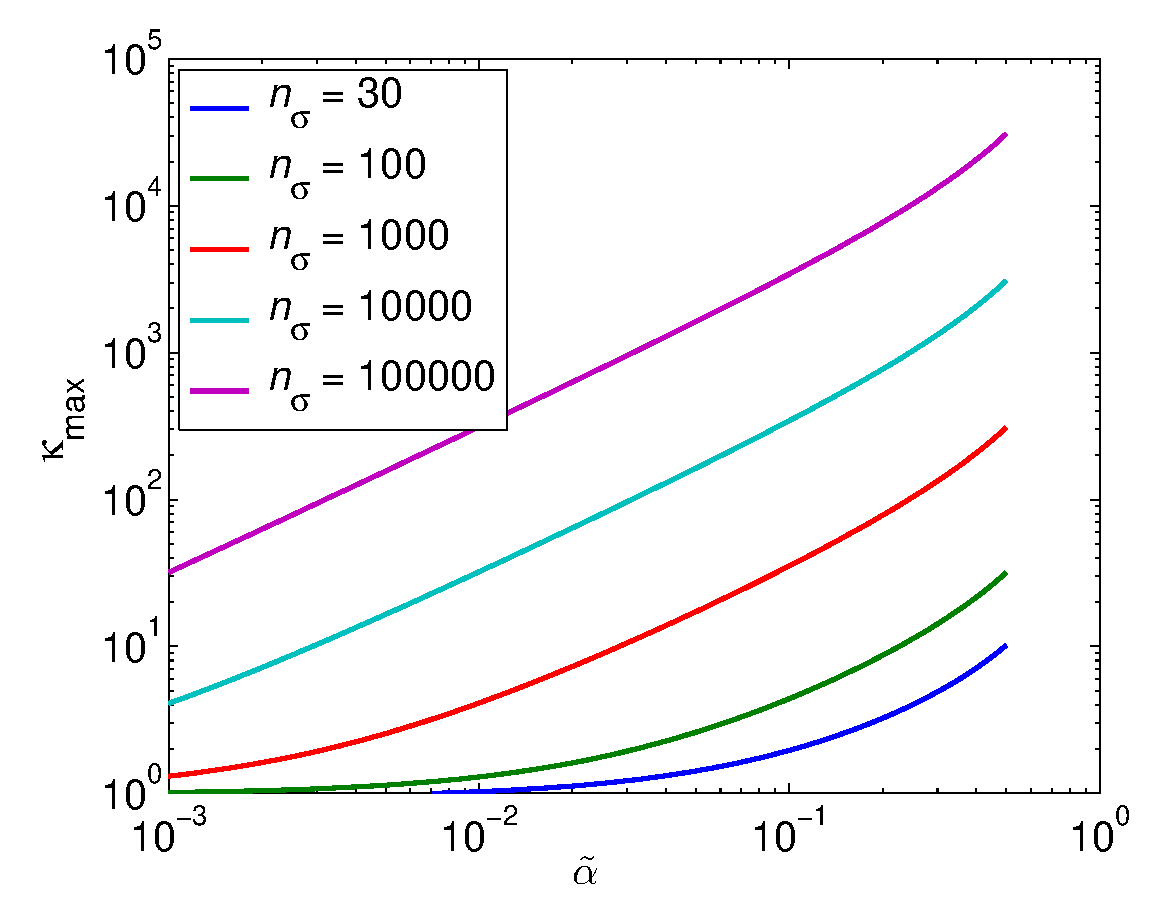
\includegraphics[width=2.1in]{kurtmaxfig} \\
% switch to kurtmaxfig.eps if not using pdflatex
(a)
\end{minipage}
\quad 
\begin{minipage}{2.1in}\centering
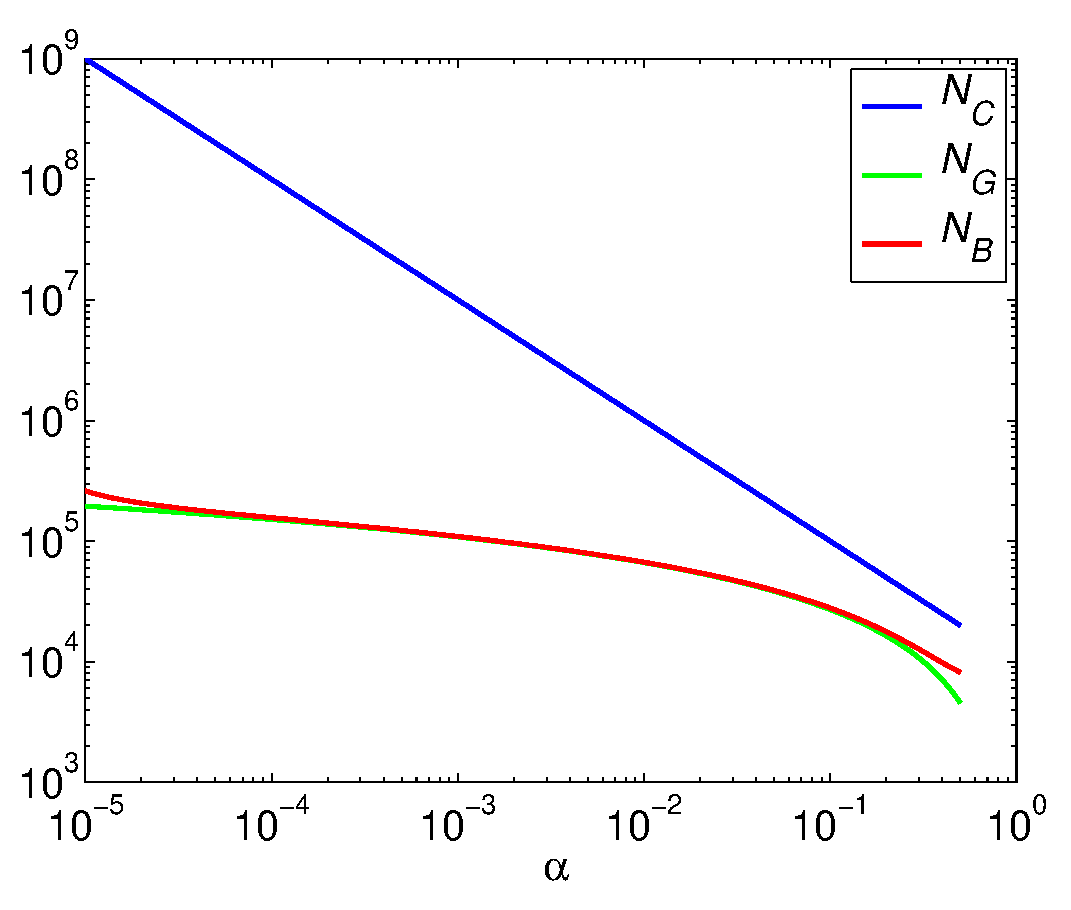
\includegraphics[width=2.1in]{alphacompare}\\
(b)
\end{minipage}
\caption{(a) The maximum kurtosis, $\kappa_{\max}(\alpha,n_{\sigma},1.5)$, as defined in \eqref{kappamaxdef}; (b) comparison of sample sizes $ N_G(0.01,\alpha)$, $N_C(0.01,\alpha)$, and $N_B(0.01,\alpha,\kappa_{\max}^{3/4}(\alpha,1000,1.5))$.\label{kurtmaxcompareNfig}}
\end{figure}

\subsection{Conservative interval widths}

Here we consider how to choose the sample size
$n$ to get the desired coverage level
from an interval with half-length at most $\varepsilon$.
We suppose here that $\sigma$ is known.  
In practice we will use a conservative (biased high) estimate
for $\sigma$.

First, if the CLT held exactly and not just asymptotically,
then we could use a CLT sample size, of
$$
N_{\mathrm{CLT}}(\varepsilon,\sigma,\alpha)
= 
% I changed the arguments of these sample size numbers to
% use \varepsilon and \sigma directly instead of
% through their ratio. It is a key fact that only the
% ratio matters. Yet I think more people will use the formula
% incorrectly if we define it via a ratio argument.
% In particular the old (13a) and (13b) defined N_C
% with argument \varepsilon for which \varepsilon/\sigma
% was inserted.  That could mix people up.  -Art
\Bigl\lceil
\Bigl(
\frac{Z^{1-\alpha/2}\sigma}{\varepsilon}
\Bigr)^2
\Bigr\rceil
$$
independent values of $Y_i$ in an interval
like the one in~\eqref{eq:99ci}.

Given knowledge of $\sigma$, but no assurance
of a Gaussian distribution for $\hat\mu_n$, we
could instead select a sample size based on
Chebychev's inequality, taking
\begin{align}\label{NCdef}
N_{\mathrm{Cheb}}(\varepsilon,\sigma,\alpha)
= 
\Bigl\lceil\frac{\sigma^2}{\alpha\varepsilon^2}\Bigr\rceil
\end{align}
observations $Y_i$ and using an interval like~\eqref{eq:99ci}
gives 
\begin{align}\label{ChebErr}
\Pr(|\hat\mu-\mu|\le\varepsilon)\ge 1-\alpha.
\end{align}
Naturally $N_{\mathrm{Cheb}}\ge N_{\mathrm{CLT}}$.

Finally, we could use the non-uniform Berry-Esseen
inequality from Theorem~\ref{thm:BE}.
This inequality requires a finite third moment
$M_3(Y) = \e(|Y-\e(Y)|^3)$. Let $\widetilde M_3 = M_3(Y)/\sigma^3$.
The non-uniform Berry-Esseen inequality implies that
\begin{align} 
\nonumber
\Prob\left[\abs{\hmu_n - \mu} <\frac{\sigma}{\sqrt{n}}x\right]&=\Prob\left[\hmu_n - \mu<\frac{\sigma}{\sqrt{n}}x\right]-\Prob\left[\hmu_n - \mu \le -\frac{\sigma}{\sqrt{n}}x\right]\\ 
% NOTE: the second one is \le not <
% equality is not necessarily a probability zero event
% because \hat\mu_n could have a discrete distribution
\nonumber
&\ge \left[\Phi(x)-\frac{0.56\widetilde{M}_3}{\sqrt{n}}(1+\abs{x})^{-3}\right] -\left[\Phi(-x) + \frac{0.56\widetilde{M}_3}{\sqrt{n}}(1+\abs{x})^{-3}\right]\\
&=1-2\left(\frac{0.56\widetilde{M}_3}{\sqrt{n}}(1+\abs{x})^{-3}+\Phi(-x)\right), \label{BEresult}
\end{align}
for all $x\in\real$.
Choosing $x=\varepsilon\sqrt{n}/\sigma$, we find that the probability of
making an error less than $\varepsilon$ is bounded below by $1-\alpha$, i.e., 
\begin{subequations} \label{proberrcritsampleBE}
\begin{equation}
\Prob[\abs{\hmu_n -\mu}<\varepsilon] \geq 1-\alpha,  \quad \text{provided } n \ge N_{\mathrm{BE}}(\varepsilon,\sigma,\alpha,\widetilde{M}_3),
\end{equation}
where the Berry-Esseen sample size is
\begin{equation}\label{NB}
N_{\mathrm{BE}}(\varepsilon,\sigma,\alpha,M) := \min \left \{ n \in \natu : \Phi\left(-\sqrt{n}\varepsilon/\sigma  \right)+\frac{0.56M}{\sqrt{n}\left(1+ \sqrt{n}\epsilon/\sigma \right)^{3}}
\le \frac{\alpha}{2} \right \}.
\end{equation}
\end{subequations}
To compute this value, we need to know
$\widetilde M_3$. In practice, substituting an upper
bound on $\widetilde M_3$ yields an upper
bound on the necessary sample size.

It is possible that in some situations
$N_{\mathrm{BE}}>N_{\mathrm{Cheb}}$ might
hold. In such cases we could use $N_{\mathrm{Cheb}}$
instead.

\subsection{Algorithm and theorem}

In detail, the two stage algorithm works
as follows.  First, the user specifies
four quantities:
\begin{itemize}
\item 
an initial sample size $n_\sigma\ge 2$
for variance estimation,
\item
a variance inflation factor $\fudge^2\in(1,\infty)$,
\item
an uncertainty tolerance $\alpha\in(0,1)$, and,
\item
an error tolerance, $\varepsilon>0$.
\end{itemize}
Though $n_\sigma$ can be as small as $2$ it should
ordinarily be larger.  


At the first stage of the algorithm,
$Y_1,\dots,Y_{n_\sigma}$ are sampled independently
from the same distribution as $Y$.
Then the variance estimate $\hat\sigma^2 = \fudge^2\hat v_{n_\sigma}$
is computed using~\eqref{eq:samplevar} to compute
$\hat v_{n_\sigma}$.

To prepare for the second stage of the algorithm
we compute $\tilde\alpha = 1-\sqrt{1-\alpha}$
and then $\tilde\kappa_{\max} = \tilde\kappa_{\max}(\tilde\alpha,n_\sigma,\fudge)$
using equation~\eqref{kappamaxdef}.
The sample size for the second stage is
\[
n = N_{\mu}(\varepsilon,\hsigma,\tilde\alpha,\tilde\kappa_{\max}^{3/4}),
\]
where
\begin{equation} \label{NCBdef}
N_{\mu}(\varepsilon,\sigma,\alpha,M) 
:= \min\bigl( N_{\mathrm{Cheb}}(\varepsilon,\sigma,\alpha), 
N_{\mathrm{BE}}(\varepsilon,\sigma,\alpha,M) \bigr).
\end{equation} 
Recall that
$N_{\mathrm{Cheb}}$ is defined in \eqref{NCdef} and  $N_{\mathrm{BE}}$ 
is defined in \eqref{NB}.  

After this preparation, the second stage is to sample
$Y_{n_\sigma+1},\dots,Y_{n_\sigma+N_\mu}$ independently
from the distribution of $Y$ and compute
\begin{align}\label{eq:theestimate}
\hat\mu = \frac1{N_\mu}\sum_{i=n_\sigma+1}^{n_\sigma+N_\mu}Y_i.
\end{align}


\begin{theorem} \label{mainadaptthm} 
Let $Y$ be a random variable with mean $\mu$.
If $\widetilde M_4(Y) \le \tilde\kappa_{\max}(\tilde\alpha,n_\sigma,\fudge)$
then the two stage algorithm above yields an estimate
$\hat\mu$ given by~\eqref{eq:theestimate} which satisfies
$$\Pr( |\hat\mu-\mu|\le\varepsilon)\ge 1-\alpha.$$
\end{theorem}
\begin{proof} 
The first stage yields a variance estimate satisfying
$
\Pr( \hsigma^2 >\sigma^2)\ge 1-\tilde\alpha
$
by \eqref{kappamaxdef} applied with error tolerance $\tilde\alpha$.
The second stage yields
$\Pr( |\hat\mu_n-\mu|\le\varepsilon)\ge 1-\tilde\alpha$
by the Berry-Esseen result~\eqref{BEresult},
so long as $\hat\sigma\ge\sigma$
and $\widetilde M_3(Y)\le \tilde\kappa_{\max}(\tilde\alpha,n_\sigma,\fudge)$.
The second condition holds under the theorem's hypothesis
because $\widetilde{M}_3 \le \tilde\kappa_{\max}^{3/4}$;
see~\eqref{eq:boundm3}.
%There are three primary random variables in this algorithm:  the estimated upper bound on the standard deviation, $\hsigma$, the sample size to estimate the mean, $n$, which is an explicit function of $\hsigma$, and the estimated mean, $\hmu_n$. By  \eqref{ChebErr} and \eqref{proberrcritsampleBE} it then follows that  $\Prob\left[\abs{\hmu_n-\mu} \le \varepsilon \right] \geq 1-\tilde\alpha$, provided that $\hsigma  \ge \sigma$. 
Thus, in the two stage algorithm we have
\begin{align*}
\Prob\left(\abs{\hmu_n-\mu} \le \varepsilon \right) &
= \e\bigl(\Prob\left(\abs{\hmu_n-\mu} \le \varepsilon \mid \hsigma \right) \bigr) \\
& \ge \e\left((1-\tilde\alpha) 1_{\sigma\le\hsigma}\right)\\
& \ge (1-\tilde\alpha) (1-\tilde\alpha) = 1-\alpha.\qedhere
\end{align*}
\end{proof}

\section{Illustrative examples}

Here we illustrate the difficulties of fixed precision
computation.  Our first example uses the two stage
algorithm from Section~\ref{sec:twostage}. 
Our second example illustrates difficulties with
the deterministic {\tt quad} function from Matlab.

\subsection{Two stage algorithm}

To illustrate our two stage algorithm, consider the following univariate step-function integrated against the uniform probability distribution on $[0,1]$, i.e., $\rho=1$:
\begin{equation} \label{exampleeq}
f(x) = \begin{cases} \mu + \sigma \sqrt{\frac{1-p}{p}}, & 0 \le x \le p,\\
\mu - \sigma \sqrt{\frac{p}{1-p}}, & p < x \le 1,
\end{cases} %\qquad \mu=\int_0^1 f(x) \, \dif x, \qquad \sigma^2=\int_0^1 [f(x)-\mu]^2 \, \dif x.
\end{equation}
where $p \in (0,1)$ is a parameter.  
%An adaptive Monte Carlo algorithm developed in the next section is able to approximate the integral well for moderate values of $p$ but not for very small ones.  
The test function parameters are $\mu=\sigma=1$.  The algorithm parameters are an absolute error tolerance of $0.01$, an uncertainty of $\alpha=5\%$, a sample size for estimating the variance of $n_\sigma=1000$, and a variance inflation factor $\fudge=1.5$.  Table \ref{stepfunexamptable} shows the percentage of times that the error tolerance is met for various values of $p$.  For $p=0.005$ the algorithm exceeds the required $95\%$ success, but for $p=0.0001$ the algorithm only gets the correct answer less than $10\%$ of the time.  Figure \ref{normalerrfig} shows the empirical distribution of the normalized error.  A normalized error no greater than one means that the error tolerance has been met.  

\begin{table}
\caption{Probability of meeting the error tolerance for test function \eqref{exampleeq} using the adaptive algorithm in Theorem \ref{mainadaptthm}. \label{stepfunexamptable}}
\[
\begin{array}{r|ccccccccccc}
p &     0.0001 &   0.0002 &   0.0005 &    0.001 &    0.002 &    0.005 & \\ 
\hline
\Prob(\abs{\mu-\hmu_n} \le 0.01)  &    8.90\% &    21.30\% &    39.80\% &    63.20\% &    85.80\% &    99.50\% & \\ 
\end{array}
\]
\end{table}

\begin{figure}
\centering
%\includegraphics[width=3in]{NormalErrFig.eps}
\caption{Empirical distribution function of $\abs{\mu-\hmu_n}/0.01$ for example \eqref{exampleeq} and  various values of $p$ using the adaptive algorithm in Theorem \ref{mainadaptthm}. \label{normalerrfig}}
\end{figure}

%The difficulty here is not a deficiency of the adaptive algorithm developed here, which is a modification of what is described above.  
%The point is that any algorithm can be fooled.  
In this case, the initial sample used to estimate the variance of the integrand may miss a very narrow spike.  Without a good estimate of this variance, there is no reliable determination of the sample size needed for computing a sample mean that is close enough to the mean of the function.  Theorem \ref{mainadaptthm} describes under what conditions this adaptive algorithm will not be fooled.
In the present example, small values of $p$ lead to large values
of $\tilde\kappa$ and for small enough $p$
the kurtosis condition in Theorem~\ref{mainadaptthm}
is violated.

\subsection{MATLAB's {\tt quad}}

The difficulties of error estimation are not unique to Monte Carlo methods. For the step function $f$ defined in \eqref{exampleeq}, MATLAB's {\tt quad} function approximates $\int_0^1 f(x - 1/\sqrt{2} \pmod 1) \, \dif x$  with an error tolerance of $10^{-14}$ to be $\approx 0.92911$, instead of the true answer of $1$.  Thus, the step function can fool automatic quadrature routines.  Figure \ref{foolquadfig} displays the integrand
\[
f(x) = 1+\cos\left(8\pi\min\left(\max\left(\frac{x-0.27158}{0.45684},0\right),1\right)\right), \qquad \int_0^1 f(x) \, \dif x = 1.54316.
\]
Here the constants $0.27158$ and $0.45684$ are chosen to fool MATLAB's {\tt quad} function.  Applying {\tt quad} to approximate the above integral with an error tolerance of $10^{-14}$ gives the answer $2$, since all of the integrand values sampled by {\tt quad} are $2$.  Thus, {\tt quad} is fooled again, even though this integrand has continuous first derivative.  

\begin{figure}
\centering
%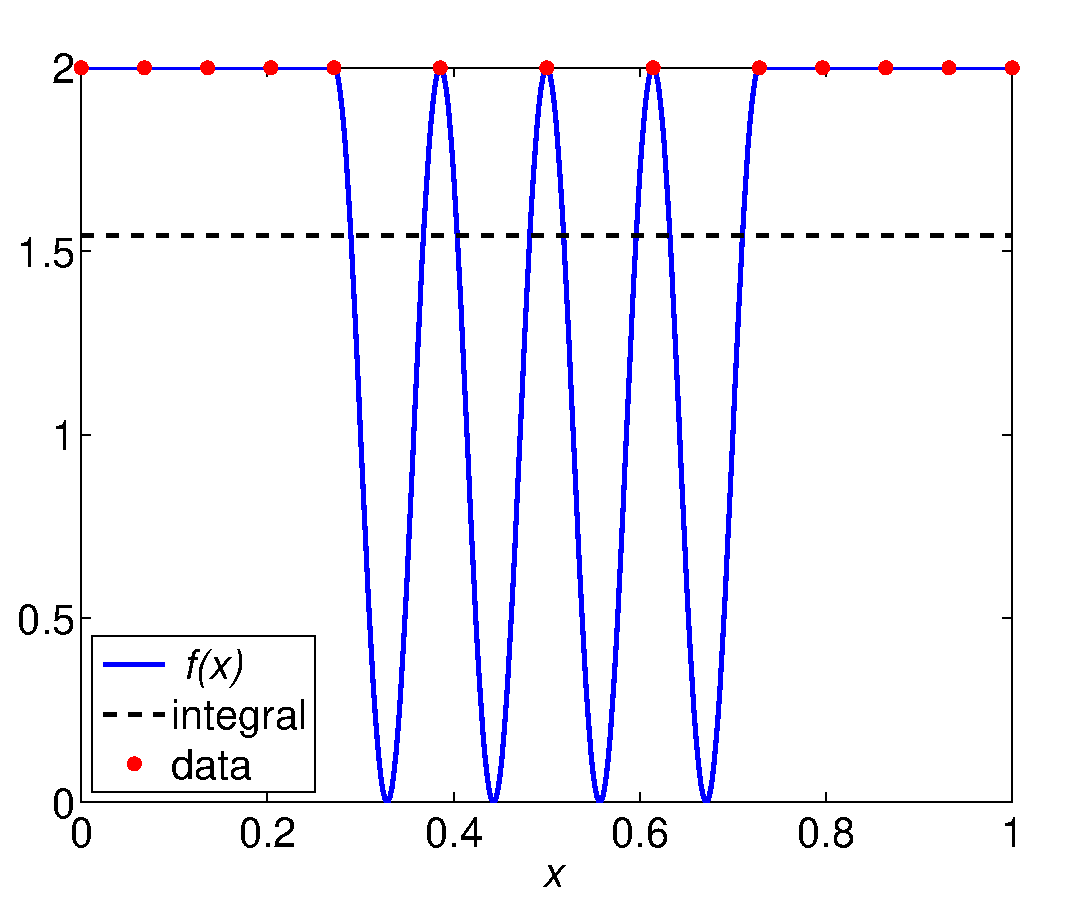
\includegraphics[width=3in]{FoolQuadFunction.eps}
\caption{Integrand that fools MATLAB's {\tt quad} function. \label{foolquadfig}}
\end{figure}

%These two examples illustrate that although quadrature rules are valuable, they may give the wrong answers.  The goal of theory is to develop quadrature rules that have iron-clad sufficient conditions for the success.   This article does so for adaptive Monte Calo rules.  Thus, the step function example will be shown to fail to satisfy those conditions when the adaptive Monte Carlo rule fails to meet the required tolerance.


\section{Algorithm cost}

\section{Relative error}

\end{document}
